% 图 1.1 元磁矩：(a) 元电流环 (b) 有限回路为无穷小电流环之和
\documentclass[tikz,border=5pt]{standalone}
\usetikzlibrary{arrows.meta,decorations.markings}
\usepackage{amsmath}
\usepackage{bm}
\usepackage{fontspec}
\setmainfont{Times New Roman}
\begin{document}
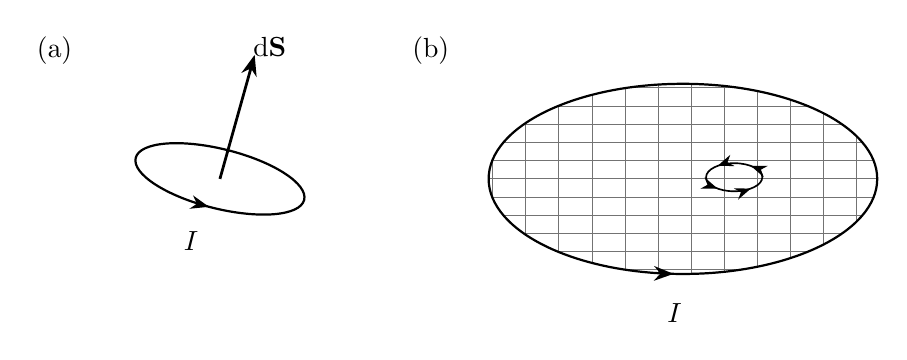
\begin{tikzpicture}[line width=0.8pt,>=Stealth,scale=1.05]
% ---------- (a) ----------
\node at (-2.0,1.55) {(a)};
% 倾斜的元电流环
\draw[rotate=-14,postaction={decorate,decoration={markings,
  mark=at position 0.74 with {\arrow[line width=0.8pt]{>}}}}]
  (0,0) ellipse (1.05 and 0.36);
% dS 矢量（回路法线）
\draw[->,line width=1.0pt] (0,0) -- (0.42,1.5)
  node[above right=-2pt,inner sep=1pt] {$\mathrm{d}\boldsymbol{\mathrm{S}}$};
\node at (-0.35,-0.75) {$I$};
% ---------- (b) ----------
\begin{scope}[shift={(5.6,0)}]
\node at (-3.05,1.55) {(b)};
% 回路内部网格（无穷小电流环阵列）
\begin{scope}
  \clip (0,0) ellipse (2.35 and 1.15);
  \foreach \x in {-2.3,-1.9,...,2.3}
    \draw[line width=0.35pt,black!55] (\x,-1.25) -- (\x,1.25);
  \foreach \y in {-1.1,-0.88,...,1.1}
    \draw[line width=0.35pt,black!55] (-2.45,\y) -- (2.45,\y);
\end{scope}
% 回路外轮廓（箭头示电流方向）
\draw[postaction={decorate,decoration={markings,
  mark=at position 0.74 with {\arrow[line width=0.9pt]{>}}}}]
  (0,0) ellipse (2.35 and 1.15);
% 中心处一个小电流环（环上四个逆时针切向箭头示环流方向）
\draw[line width=0.6pt,postaction={decorate,decoration={markings,
  mark=between positions 0.125 and 0.875 step 0.25 with
    {\arrow[line width=0.6pt]{Stealth}}}}] (0.62,0.02) ellipse (0.34 and 0.17);
\node at (-0.1,-1.62) {$I$};
\end{scope}
\end{tikzpicture}
\end{document}
